% Chapter 2

\chapter{Background} % Main chapter title

\label{chap:Background} % For referencing the chapter elsewhere, use \ref{chap:Chapter2} 

%----------------------------------------------------------------------------------------

\section{Distributed Systems}

In the early days of computing, computers were large and expensive, operating as standalone machines without the ability to communicate with each other. As technology advanced, smaller and more affordable computers, such as smartphones and other devices, were developed, along with high-speed networking that allowed connectivity across a network \cite{Tanenbaum2023}. These innovations made it possible to create systems distributed across nodes where tasks could be processed collectively to achieve a common goal \cite{Tanenbaum2023}. Nodes in a distributed system may refer to physical devices or software processes \cite{Vitillo2021}.


To the end-user, distributed systems appear as a single, large virtual system, making the underlying logic transparent \cite{Vitillo2021}. These systems achieve a shared objective by transmitting messages through various nodes and dividing computational tasks among them, increasing resilience and isolating business logic \cite{Sari2015, Vitillo2021}. Distributed systems can present heterogeneity, such as differing clocks, memory, programming languages, operating systems, or geographical locations, all of which must be abstracted from the end-user \cite{Sari2015, Tanenbaum2023}.

\subsection{Characteristics}

On a distributed system, when being well-structured, it is possible to find, among others, the following most popular characteristic:

\subsubsection{Transparency}

Transparency in distributed systems enables seamless user interaction by hiding the complexity of underlying operations \cite{Tanenbaum2023, Ledmi2018}. Key aspects include access transparency, which allows resource usage without concern for system differences, and location transparency, which hides the physical location of resources, as seen with the \glspl{URL} \cite{Tanenbaum2023, Coulouris2012}. Replication transparency ensures reliability by masking data duplication, while failure transparency enables systems to handle faults without user disruption \cite{Tanenbaum2023, Coulouris2012}. Together, these forms of transparency enhance usability, robustness, and reliability.

\subsubsection{Reliability and Availability}

A distributed system should have reliability and availability aspects. Reliability refers to its ability to continuously perform its intended requirements without interruption, operating exactly as designed, even in the presence of certain internal failures \cite{Ahmed2013}. A highly reliable system maintains consistent, uninterrupted service over an extended period, minimizing disruptions for users \cite{Tanenbaum2023}. On other hand, availability measures the probability that the system is operational and ready to respond correctly at any given moment, often expressed as a percentage of system up-time \cite{Tanenbaum2023, atlassian-availability}.

\subsubsection{Scalability}

Designing and building a distributed system is complex, but also enables the creation of highly scalable systems, capable of expanding to meet increasing demands \cite{Tanenbaum2023, Vitillo2021, Valkov2018}. This characteristic is particularly evident as cloud-based systems become more popular, allowing users to interact with applications over the internet rather than relying on local desktop computing power \cite{Lindsay2021}. Cloud services must support a large volume of simultaneous connections and interactions, making scalability a crucial factor \cite{Tanenbaum2023}.

\subsubsection{Fault tolerance}

Fault tolerance is a critical characteristic of distributed systems, closely linked to reliability, availability, and scalability. For a system to maintain these properties, it must be able to mask failures and continue operating despite the presence of errors \cite{Tanenbaum2023}. Fault tolerance is especially vital in distributed environments where system failures can lead to significant disruptions and economic losses across sectors such as finance, telecommunications, and transportation \cite{Sari2015}.

The primary goal of a fault-tolerant system is to enable continuous operation by employing specific strategies and design patterns to mask the possible errors \cite{Kleppmann2017}.

\subsection{Communication}

Communication is fundamental in distributed systems for coordination and data exchange. Nodes communicate over networks or via \gls{IPC} when on the same machine \cite{Vitillo2021}. Synchronous communication involves blocking operations where the sender waits for a response, suitable for scenarios requiring confirmation \cite{Tanenbaum2023, Coulouris2012}. In contrast, asynchronous communication allows non-blocking operations, enabling the sender to proceed without waiting. This approach, often supported by message queues, is a good suit for decoupled and heterogeneous systems \cite{Tanenbaum2023}.

\subsection{Challenges}

Distributed systems encounter numerous challenges, including scalability \cite{Ahmed2013}, managing software, network, and disk failures \cite{Naik2021, aws-challenges-dist-sys}, heterogeneity \cite{Coulouris2012}, coordination among nodes, and difficulties on debugging and testing \cite{Vitillo2021, aws-challenges-dist-sys}. For the scope of this dissertation only the CAP theorem will be discussed.

\textbf{CAP Theorem.} The CAP theorem says that in a system where nodes are networked and share data, it is impossible to simultaneously achieve all three properties of Consistency, Availability, and Partition Tolerance \cite{Tanenbaum2023, Vitillo2021}. This theorem underlines a critical trade-off in distributed systems: only two of these properties can be fully ensured at any given time \cite{ibm-cap-theorem}. A description of the properties can be given by:

\begin{itemize}
    \item \textbf{Consistency:} Ensures that all nodes in the system reflect the same data at any time, so each read returns the latest write.
    \item \textbf{Availability:} Guarantees that every request receives a response, whether successful or not, even if some nodes are offline.
    \item \textbf{Partition tolerance:} Allows the system to continue operating despite network partitions, where nodes may temporarily lose the ability to communicate.
\end{itemize}

According to the CAP theorem, when a network partition occurs, a distributed system must prioritize either consistency or availability, as achieving all three properties is not feasible in practice \cite{Tanenbaum2023, ibm-cap-theorem, Vitillo2021}. This concept is directly relevant to this dissertation, as fault tolerance strategies discussed later, like replication and redundancy, will account for these trade-offs to optimize specific properties.

%%%%%%%%%%%%%%%%%%%%%%%%%%% FAULT TOLERANCE %%%%%%%%%%%%%%%%%%%%%%%%%%%

\section{Fault Tolerance}

With the extensive use of software systems across various domains, the demand for reliable and available systems is essential. However, errors in software are inevitable, making fault tolerance a critical attribute for systems to continue functioning correctly even in the presence of failures \cite{Sari2015}. Fault tolerance can address a range of issues, including networking, hardware, software, and other dimensions, with various strategies designed to manage these different fault types \cite{Tanenbaum2023,Noor2019}.

\subsection{Fault Tolerance Taxonomy}

Firstly, it is important to classify and understand the types of failures that can arise. This section presents a taxonomy of fault tolerance concepts, drawing on the framework proposed by \textcite{Isukapalli2024}. A fault, which types are summarized in the Table \ref{tab:faults_types}, is defined as an underlying defect within a system component that can lead to a failure, which is a deviation from the intended internal state. If this error remains unresolved, it may escalate into a system failure, potentially impacting system functionality either partially or completely \cite{Isukapalli2024,Reghenzani2023}.

\begin{table}[h!]
    \centering
    \begin{tabular}{|l|p{11.3cm}|}
        \hline
        \textbf{Type of Fault} & \textbf{Description}                                                                                                                                                                                \\ \hline
        Transient Faults       & Temporary conditions like network issues or service unavailability. Can typically be resolved by restarting the application when the underlying condition is fixed \cite{Isukapalli2024}.           \\ \hline
        Intermittent Faults    & Unpredictable symptoms related to system or hardware malfunction. Difficult to detect during testing and emerge during system operation, and also hard to completely resolve \cite{Isukapalli2024}. \\ \hline
        Permanent Faults       & Persistent issues that continue until the root cause is identified and addressed. Relatively straightforward to fix, typically related to complete component malfunction \cite{Tanenbaum2023}.      \\ \hline
        Byzantine Faults       & Caused by internal system state corruption or incorrect network routing. Handling is complex and costly, often requiring multiple component replicas and voting mechanisms \cite{Isukapalli2024}.   \\ \hline
    \end{tabular}
    \caption{Brief description of fauls types}
    \label{tab:faults_types}
\end{table}

Failures are the external manifestations of the internal faults, as outlined in Table \ref{tab:failure_types}. These include crash failures, where the system halts entirely, to arbitrary failures, where responses are erratic and potentially misleading \cite{Tanenbaum2023}.

\begin{table}[h!]
    \centering
    \begin{tabular}{|l|p{11.3cm}|}
        \hline
        \textbf{Type of Failure} & \textbf{Description}                                                                                                                                                                                  \\ \hline
        Crash Failure            & The system halts and stops all operations entirely. Although it was functioning correctly before the halt, it does not resume operations or provide responses after the failure \cite{Tanenbaum2023}. \\ \hline
        Omission Failure         & The system fails to send or receive necessary messages, impacting communication and task coordination \cite{Isukapalli2024}.                                                                          \\ \hline
        Timing Failure           & The system’s response occurs outside a specified time interval, either too early or too late, causing issues in time-sensitive operations \cite{Isukapalli2024}.                                      \\ \hline
        Response Failure         & The system provides incorrect outputs or deviates from expected state transitions, potentially leading to wrong results \cite{Tanenbaum2023}.                                                         \\ \hline
        Arbitrary Failure        & The system produces random or unpredictable responses at arbitrary times, potentially with incorrect data. This type of failure is challenging to diagnose and manage \cite{Tanenbaum2023}.           \\ \hline
    \end{tabular}
    \caption{Brief description of failure types}
    \label{tab:failure_types}
\end{table}

\subsection{Strategies}

Various strategies and mechanisms can be applied to a system to achieve fault tolerance, and these must be chosen to suit the specific system type. This dissertation will primarily focus on software fault tolerance strategies that are suitable for the programming languages bellow presented. Therefore, next it will be shown some strategies that it will serve as a theoretical basis for some of techniques that it will be used.

\subsubsection{Retry Mechanism}

The retry mechanism is a widely adopted and straightforward technique that involves reattempting a failed operation under the assumption that transient faults may resolve over time \cite{Ledmi2018}. Despite its simplicity, this strategy is highly suitable in many scenarios, particularly when implementing more complex fault tolerance mechanisms would introduce unnecessary cost in environments with a high likelihood of transient faults. However, it is crucial to recognize that retrying in the case of a permanent error is pointless. Moreover, if the failure is caused by system overload, uncontrolled retries can aggravate the issue. To address these challenges, implementing a maximum retry limit and incorporating strategies such as exponential backoff, where retries are spaced out with increasing delays, becomes essential \cite{Kleppmann2017,Vitillo2021}.

This approach operates by attempting the operation a predefined number of times or until a set timeout is reached. If the retries ultimately fail, the system can fallback on alternative measures, such as logging the failure, invoking a fallback operation, or redirecting the request to another asset \cite{Isukapalli2024}. These measures ensure that in the event of a persistent fault, the system will make controlled attempts and try to fallback in a safe manner.

The retry mechanism’s simplicity and low implementation overhead make it ideal for scenarios where the cost of a retry is insignificant compared to the complexity of alternative solutions. It is particularly effective in network communication, where transient issues such as dropped packets or server unavailability often resolve with subsequent attempts \cite{Isukapalli2024}. In case of an unresolved situation it is created an omission failure due to the missing communication. Additionally, it is well-suited for database systems to handle transient locking or deadlock conditions, as well as in microservice architectures, where downstream services may temporarily become unresponsive but recover shortly thereafter \cite{Kleppmann2017}.

This strategy aligns effectively with Actor Models due to their inherent monitoring capabilities, which detect errors and initiate retries automatically. Frameworks such as Akka with Scala have built-in support for this mechanism \cite{Isukapalli2024}.

\subsubsection{Circuit Breaker Pattern}

The Circuit Breaker pattern, inspired by electrical circuits, is designed to prevent the failure of a single subsystem from cascading and compromising an entire system. This pattern tries to maintain the overall system stable by isolating failing components \cite{Vitillo2021}. By actively monitoring the health of operations and selectively blocking problematic ones, circuit breakers act as safeguards against system overload and degradation \cite{fowler-circuit-breakers}.

Circuit breakers operate in three primary states: Closed, Open, and Half-Open \cite{Vitillo2021, fowler-circuit-breakers}. In the Closed state, illustrated in Figure \ref{fig:circuit-breaker} by the first request, operations proceed as usual, with all requests passing through the circuit breaker while it monitors for potential failures. When failures exceed a predefined threshold within a specified time window, whether measured as a count or a percentage of failed attempts, the circuit breaker transitions to the Open state, illustrated in Figure \ref{fig:circuit-breaker} by the third request. In this state, all requests are blocked to prevent higher pressure on the failing subsystem. During this time, it is essential to issue an alert to monitoring systems to ensure operational visibility \cite{Vitillo2021, fowler-circuit-breakers}. After a cool-down period, the circuit breaker moves to the Half-Open state, where it permits a limited number of test requests to verify if the underlying issue has been resolved. If these test requests succeed, the circuit breaker resets to the Closed state and resumes normal operation. Otherwise, it reverts to the Open state \cite{fowler-circuit-breakers}.

\begin{figure}
    \centering
    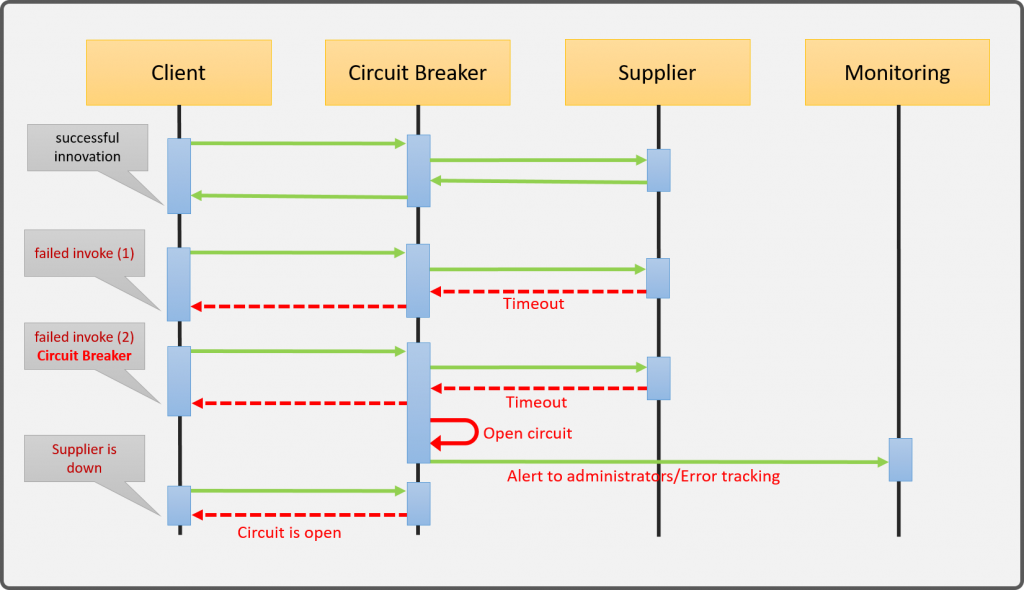
\includegraphics[width=\linewidth]{ch-background/assets/circuit-breaker.png}
    \caption[Diagram illustrating the states of a Circuit Breaker]{Diagram illustrating the states of a Circuit Breaker \footnotemark.}
    \label{fig:circuit-breaker}
\end{figure}
\footnotetext{From Oscar Blancarte Blog. \url{https://www.oscarblancarteblog.com/2018/12/04/circuit-breaker-pattern/} (accessed 4 January 2025).}

The Circuit Breaker pattern is particularly well-suited for distributed systems, such as microservice architectures, where dependencies on external services can lead to cascading failures \cite{fowler-circuit-breakers}. For instance, if a downstream service becomes unresponsive, the circuit breaker blocks further requests, providing the service with time to heal and avoiding the risk of overloading it with retries \cite{Vitillo2021}. It is equally effective in scenarios involving a third-party \gls{API}, where temporary rate limits or outages can impact availability. In database systems, circuit breakers can mitigate the effects of resource contention or extended downtime by isolating problematic queries, ensuring the broader system remains operational.

When compared to pure retry mechanisms, the Circuit Breaker pattern provides a more sophisticated approach to fault tolerance. While retries focus on recovering from transient faults, they can harm even more issues under conditions such as system overload or persistent failures \cite{Vitillo2021}. In contrast, circuit breakers proactively block failing operations, reducing the risk of cascading failures and preserving overall system stability.

\subsubsection{Replication and Redundancy}

Replication is a fundamental strategy for achieving fault tolerance in distributed systems and is widely used across various domains \cite{Sari2015}. By creating multiple replicas of data or processes, replication eliminates single points of failure, ensuring system reliability, availability, and transparency \cite{Coulouris2012}. This approach allows a system to tolerate faults by introducing redundancy, which distributes operations across a group of replicas rather than relying on a single vulnerable node \cite{Tanenbaum2023}.

To effectively coordinate replicas and maintain consistency, replication mechanisms employ various strategies, which can be categorized as follows \cite{Isukapalli2024}:

\begin{itemize}
    \item	\textbf{Active Replication (Semi-Active):} In this strategy, all replicas process incoming requests simultaneously, and the system relies on consensus algorithms to maintain consistency among the results.
    \item	\textbf{Passive Replication (Semi-Passive):} One replica, designated as the leader or primary, handles all client requests and updates other replicas with state information. In case of a primary failure, backup replicas are promoted or synchronized to restore the system’s functioning.
    \item	\textbf{Passive Backup (Fully Passive):} Replicas act as standby backups in this approach. A backup replica is only activated when the primary fails, minimizing overhead during normal operation.
\end{itemize}

These replication strategies align with the principles of the CAP theorem, which states that a distributed system can guarantee at most two of the following three properties: consistency, availability, and partition tolerance. Replication strategies often emphasize availability and partition tolerance, potentially compromising consistency due to the inherent challenges of achieving consensus and synchronizing data across replicas. Nonetheless, this trade-off enables systems to scale, increase availability, and provide transparency to end users \cite{Kleppmann2017}.

\textbf{Consensus Algorithms}

Achieving consensus is essential in distributed systems to ensure that a group of processes operates cohesively as a single entity \cite{Tanenbaum2023}. Consensus algorithms enable replicas to agree on a shared state or a sequence of operations, even in the presence of faults. Two famous used consensus algorithms in distributed systems are Raft and Paxos \cite{Tanenbaum2023}.

\textit{\underline{Paxos}}

Paxos appeared in 1989 and has evolved over time, earning a reputation as a complex and difficult to understand algorithm \cite{Tanenbaum2023}. Due to its challenges and the emergence of newer alternatives like Raft, which is described below, this explanation of Paxos will concentrate on its core concepts without going into exhaustive detail.

Paxos ensures that a group of distributed replicas agrees on a single value, even in the presence of faults. It operates under challenging conditions: replicas may crash and recover, messages can be delayed, reordered, or lost, and no assumptions are made about message delivery timing \cite{Howard2020, Tanenbaum2023}. The algorithm revolves around three distinct roles \cite{Coulouris2012, Howard2020}:

\begin{itemize}
    \item \textbf{Proposers:} Suggest values for the system to agree upon.
    \item \textbf{Acceptors:} Vote on proposals, ensuring fault tolerance by requiring a majority for decisions.
    \item \textbf{Learners:} Observe the final agreed value and disseminate the result across the system.
\end{itemize}

With the roles defined, the Paxos algorithm progresses through the following phases to achieve consensus \cite{Tanenbaum2023, Coulouris2012, Howard2020}:

\begin{itemize}
    \item \textbf{Prepare Phase:}
          A proposer generates a proposal with a unique sequence number and sends a \emph{prepare request} to a list of acceptors.
          \begin{itemize}
              \item Acceptors respond with a \textit{promise} not to accept earlier proposals.
              \item If an acceptor has already accepted a value, it shares this value with the proposer.
          \end{itemize}

    \item \textbf{Accept Phase:}
          Based on responses from the prepare phase, the proposer sends an \textit{accept request} with a value:
          \begin{itemize}
              \item If an acceptor had previously accepted a value, the proposer adopts that value.
              \item Otherwise, the proposer chooses its own value.
              \item Acceptors respond by accepting the value if it doesn’t conflict with their earlier promises.
          \end{itemize}

    \item \textbf{Commit or Learn Phase:}
          Once a majority of acceptors accepts the value, consensus is achieved.
          \begin{itemize}
              \item The proposer informs all replicas, which then commit the value.
          \end{itemize}
\end{itemize}

While Paxos is robust in theory and guarantees consistency, its complexity and subtle behaviors make it difficult to implement correctly or faithfully to its original design \cite{Tanenbaum2023}. Over time, new variations and extensions, such as Multi-Paxos, have been developed. Multi-Paxos enables the system to achieve consensus on multiple values, making it more practical for real-world applications, like Chubby lock service of Google \cite{Coulouris2012}, but in general it is not considered a highly adopted algorithm.

The inherent complexity of Paxos has also driven the creation of simpler consensus algorithms, such as Raft, which aim to provide the same guarantees while being easier to understand and implement \cite{Tanenbaum2023, Howard2020}.

\textit{\underline{Raft}}

Raft is a consensus protocol designed to enable fault-tolerant operation in distributed systems. It ensures that a process will eventually detect if another process has failed and take appropriate corrective action. Raft was developed as a more comprehensible and practical alternative to Paxos, addressing its complexity and promoting clarity \cite{raft-diego,Tanenbaum2023}. This algorithm fits on semi passive replication strategy.

Each process in Raft maintains a log of operations, which may include both committed and uncommitted entries. The primary goal of Raft is to ensure that these logs remain consistent across all servers, such that committed operations appear in the same order and position in every log \cite{Tanenbaum2023}. To achieve this, Raft uses a leader-based approach, where one server assumes the role of leader while the remaining servers act as followers. The leader is responsible for determining the sequence of operations and ensuring their consistent replication \cite{Vitillo2021}. The typical number of nodes used is five \cite{raft-diego}.

When a operation request is submitted, the leader appends the operation to its log as a tuple where it contains: the operation to be executed, the current term of the leader, and the index of the operation in the leader's logs \cite{Tanenbaum2023}. The term is reset every time an election occurs, starting from zero \cite{raft-diego}. This information is then propagated to the followers using a process inspired by the two-phase commit protocol, where it consists on \cite{Tanenbaum2023,Vitillo2021}:
\begin{enumerate}
    \item \textbf{Append Phase:} The leader sends the new log entry to all followers. The followers append the entry to their logs and send an acknowledgment signal back to the leader.
    \item \textbf{Commit Phase:} Upon receiving the acknowledgments from a majority of followers, the leader marks the entry as committed, executes the operation, updates its state, and notifies the client of the result. At the same time, the leader informs all followers of the commitment, ensuring their logs reflect the updated status.
\end{enumerate}

This two-step process guarantees that committed entries are replicated on a majority of servers, preserving durability and consistency, even in case of server failures \cite{Tanenbaum2023}. However, there are cases where the leader fails and an election starts among the followers. The followers acknowledge the leader’s failure through the heartbeat strategy, where after a certain time without receiving any signal sent by the leader, the follower starts an election \cite{Vitillo2021,raft-diego}, like represented on Figure \ref{fig:state-raft} by the change of state from follower to candidate. To prevent multiple followers from initiating elections simultaneously, heartbeat timeouts are randomized \cite{Vitillo2021, Tanenbaum2023}.


The change of state of the node is displayed on the Figure \ref{fig:state-raft} and the process consists on the following steps \cite{Vitillo2021,raft-diego}:
\begin{enumerate}
    \item 	\textbf{Transition to Candidate:} A follower transitions to a candidate state, increments its term number, and broadcasts requests for votes from other servers.
    \item 	\textbf{Voting:} Each server can vote for one candidate per term. A server grants its vote only if the candidate’s log is at least as complete as its own, ensuring that the elected leader has the most up-to-date log.
    \item 	\textbf{Leader Selection:} If a candidate receives votes from a majority of servers, it becomes the leader for the current term.
\end{enumerate}

Once elected, the new leader reconciles any inconsistencies by broadcasting missing log entries to followers during subsequent operations, ensuring consistency across the cluster \cite{Tanenbaum2023}.

\begin{figure}
    \centering
    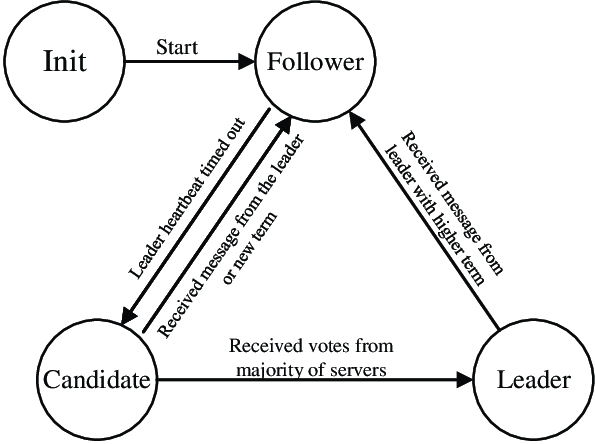
\includegraphics[scale=1]{ch-background/assets/state-raft.png}
    \caption[Diagram illustrating the states of a node in the Raft algorithm]{Diagram illustrating the states of a node in the Raft algorithm \footnotemark.}
    \label{fig:state-raft}
\end{figure}
\footnotetext{Adapted from Jinjie Xu and colleagues. \url{https://doi.org/10.3390/sym14061122/} (accessed 4 January 2025).}

Raft’s structured and modular design prioritizes simplicity, reliability, and fault tolerance. Its leader-based model centralizes decision-making and log synchronization, while its robust mechanisms for log replication and leader election ensure consistency and availability even in the face of failures.

\textit{\underline{Comparison of Paxos and Raft}}

Both Paxos and Raft are leader-based distributed consensus algorithms designed to ensure consistency in replicated state machines \cite{Howard2020}. The key difference lies in their approach to leader election and log replication. Raft prioritizes simplicity and readability, requiring candidates to have up-to-date logs before becoming leaders, avoiding complex log synchronization steps common in Paxos. Paxos, while general and flexible, allows for greater complexity, such as out-of-order log replication and term adjustments during leadership changes \cite{Tanenbaum2023}.

Raft is widely used in distributed systems requiring high availability and consistent state management. Notable applications use adaptations of Raft, including etcd for distributed key-value storage, Consul for service discovery, and CockroachDB for scalable, consistent databases \cite{Howard2020,Vitillo2021}. Paxos, on the other hand, is often found in legacy systems and specialized applications like Google’s Chubby service \cite{Howard2020}.

\subsubsection{Check-pointing and Message Logging}

When an error compromises the system’s state, recovery actions must be taken. These strategies focus on fault recovery by addressing errors after they occur. Their primary goal is to restore the system to an state without error. Recovery strategies are generally classified as either backward recovery or forward recovery \cite{Tanenbaum2023}.

Forward recovery seeks to return the system to a correct state after it has entered an erroneous one. However, this approach requires prior knowledge of potential errors to execute fixes, which can be challenging or even unreliable \cite{Tanenbaum2023}. Alternatively, backward recovery involves periodically saving the system’s state and restoring it to the last known correct state when issues arise. This approach uses checkpoints, which are recorded snapshots of the system state that enables the recovery process \cite{Tanenbaum2023}.

Check-pointing is a backward recovery technique. It periodically saves the state of a process, enabling it to restart from the last saved state in the event of a failure. However, this approach is computationally expensive and introduces performance overhead \cite{Tanenbaum2023,Isukapalli2024}. Furthermore, some operations are inherently irreversible, which limits the effectiveness of this strategy \cite{Tanenbaum2023,Ledmi2018}. 

To address the performance overhead of check-pointing, a lighter approach, message logging, has been developed. This strategy involves maintaining a log of action messages of the system. By replaying these messages in the correct order, the system can recover to a consistent state without the need to record its entire state continuously \cite{Isukapalli2024,Ledmi2018}. Although checkpoints are still required to avoid replaying all messages from the beginning, the overhead is significantly reduced compared to traditional check-pointing \cite{Isukapalli2024}. For this strategy to work effectively, system operations must be deterministic, ensuring that replaying messages reproduces the correct state, which is also a limitation or even an impossibility in some cases \cite{Tanenbaum2023}.

Apache Flink employs check-pointing to recover state and stream positions, ensuring that the application maintains consistent semantics even in the event of failures, as outlined in the project's documentation \cite{apache-flick}. However, these strategies can be resource-intensive, and it is crucial to carefully evaluate their suitability.

\subsubsection{Overview of Fault Tolerance Strategies}

Fault tolerance is essential to ensure reliability and performance. Four key strategies have been explored, each suitable for specific scenarios of varying complexity. Retry mechanisms are a simple but effective way of dealing with transient failures such as network interruptions. For example, in an e-commerce platform, retrying a failed payment gateway request can often resolve temporary connectivity issues. In microservices, retries can be enhanced with circuit breakers that temporarily halt requests to unstable services to prevent cascading failures, such as when a downstream service becomes overloaded. For critical scenarios where fault transparency is essential, replication is more appropriate. For example, in distributed databases, replication ensures data availability even if a node fails, providing resilience for applications such as online banking or real-time analytics. Check-pointing and message logging, on the other hand, are ideal for systems where restarting is costly or inefficient. In resource-intensive processes such as \gls{AI} model training or large-scale simulations, check-pointing could allow the system to recover from the last point of progress, rather than starting from scratch and losing all data.


%%%%%%%%%%%%%%%%%%%%%%%%%%% Distributed Programming Languages %%%%%%%%%%%%%%%%%%%%%%%%%%%


\section{Distributed and Concurrency Programming}

Distributed and concurrent programming plays an important aspect in building resilient and fault-tolerant systems \cite{Armstrong2013}. In distributed systems, where components operate across multiple nodes, and in concurrent systems, where tasks can execute in parallel or concurrently on the same machine's \gls{CPU}, programming languages must provide mechanisms to manage faults effectively. These mechanisms should isolate faults to prevent cascading failures, at the same time ensuring overall system reliability and availability \cite{Nystrom2009}, or should have forms to equip the language with capacities to handle this type of systems by frameworks or libraries.

The evolution of distributed programming languages help to address the complexities of developing distributed systems, which include issues such as concurrency, parallelism, fault tolerance, and secure communication \cite{Armstrong2013}. This has driven the evolution of new paradigms, languages, frameworks, and libraries aimed at reducing development complexity in distributed and concurrent systems \cite{Valkov2018}.

\subsection{Models and Paradigms}

The field of distributed programming has been shaped by research and development in concurrency and parallelism, and some models and paradigms have been developed to address this challenge. Some ideas had some focus restricted to the research others have been addressed to the industry. In the following it will be described the models and paradigms that bring interest to this dissertation:

\subsubsection{Actor Model}

The Actor Model, a conceptual framework for concurrent and distributed computing, was introduced by Carl Hewitt in 1973 \cite{Hewitt1973}. It defines a communication paradigm where an actor, the fundamental unit of computation, interacts with other actors exclusively through asynchronous message passing, with messages serving as the basic unit of communication \cite{Trinder2017}. Each actor is equipped with its own mailbox, which receives messages and processes them sequentially \cite{Koster2016}.

A core principle of the Actor Model is isolation, maintaining their own internal state that is inaccessible and immutable by others \cite{Koster2016}. This eliminates the need for shared memory, reducing complexity and potential data races \cite{Valkov2018}.

The Actor Model also introduces the concept of supervision, where actors can monitor the behavior of other actors and take corrective actions in the event of a failure. This supervisory mechanism significantly enhances fault tolerance, enabling systems to recover gracefully from errors without compromising overall reliability \cite{Trinder2017}.

The Actor Model has been instrumental in shaping distributed system design and has been natively implemented in programming languages such as Erlang, Clojure and Elixir \cite{Randtoul2022}. Additionally, the model has been extended to other languages through frameworks and libraries. For instance, Akka brings actor-based concurrency to Java, Scala, C\texttt{\#} and F\texttt{\#} while Kilim provides similar functionality specifically for Java \cite{Trinder2017}. Comparable patterns can also be adopted in other languages like Go, Rust, and Ruby using libraries or custom abstractions.

\subsubsection{Communicating Sequential Processes}

The field of distributed computing emphasizes mathematical rigor in algorithm analysis, with one of the most influential models being \gls{CSP}, introduced by C.A.R. Hoare in 1978 \cite{Hoare1978}.

\gls{CSP} offers an abstract and formal framework for modeling interactions between concurrent processes through channels, which serve as the communication medium between them \cite{Paduraru2018}. Processes operate independently, but they are coupled via these channels, and communication is typically synchronous, requiring the sender and receiver to synchronize for message transfer \cite{Hoare1978}. While similar in some respects to the Actor Model, \gls{CSP} distinguishes itself through its emphasis on direct coupling via channels and synchronization.

The \gls{CSP} model influenced on programming languages and frameworks. For example, Go integrates \gls{CSP} concepts in its implementation of goroutines and channels \cite{go-docs, Valkov2018,Paduraru2018}. In addition, the language Occam attempts to offer a direct implementation of \gls{CSP} principles with its focus on critical projects such as satellites \cite{Brolos2021}.

\subsubsection{Microservices Architectures}

A significant evolution in designing distributed systems has emerged with the appearance of microservices architectures. This paradigm elevates the focus to a higher level of abstraction, enabling language-agnostic systems by decomposing a monolithic application into a collection of loosely coupled, independently deployable services, each responsible for a specific function \cite{Jamshidi2018}. These services communicate using lightweight protocols such as \gls{HTTP}, \gls{gRPC}, or message queues, promoting separation of concerns, modularity, scalability, and fault tolerance \cite{Jamshidi2018}.

Microservices architectures allow general-purpose programming languages to participate in distributed computing paradigms by leveraging frameworks, libraries, and microservices principles \cite{Guidi2017}.

Although microservices are often associated with strict business principles, their abstract concepts can be adapted to focus on architectural designs that leverage communication middleware for distributed communication. By adopting these principles, it becomes possible to create distributed systems with fault-tolerant capabilities using general-purpose programming languages.


\subsection{Distributed and Concurrent Programming Languages}

Distributed and concurrent programming languages are designed to handle multiple tasks simultaneously across systems or threads. Some languages, such as Java, Rust, and lower-level languages like C with PThreads, require developers to explicitly manage concurrency \cite{Valkov2018,Paduraru2018}. These approaches often introduce complexity, increasing the probability of deadlocks or race conditions. This has driven the need for languages and frameworks that abstract away these challenges, offering safer and more developer-friendly concurrency models \cite{Valkov2018}.

One widely adopted paradigm for mitigating concurrency issues is the Actor Model. By avoiding shared state and using message passing for communication, the Actor Model reduces risks inherent in traditional concurrency mechanisms such as mutexes and locks \cite{Valkov2018}. Erlang, for instance, is renowned for its fault tolerance and “let-it-crash” philosophy \cite{Armstrong2013}. Supervising actors monitor and recover from failures, making Erlang highly suitable for building robust distributed systems \cite{Armstrong2013}. Building on Erlang’s foundation, Elixir introduces modern syntax and developer tooling while retaining Erlang’s strengths for creating large-scale, fault-tolerant systems. These features make Elixir a popular choice for modern distributed systems development \cite{Juric2024}.

Haskell, a pure functional programming language, provides a deterministic approach to concurrency, ensuring consistent results regardless of execution order \cite{Valkov2018}. Its extension Cloud Haskell\footnote{Cloud Haskell: \url{https://haskell-distributed.github.io/} (accessed 4 January 2025)}, builds upon the Actor Model, drawing inspiration from Erlang, to allow distributed computation through message passing.

Similarly, Akka, a framework built for Scala, adopts the Actor Model to support distributed and concurrent applications. Akka combines Scala’s strengths in functional and object-oriented programming, enabling developers to merge these paradigms effectively \cite{Valkov2018}. Unlike Erlang, Akka operates on the \gls{JVM}, providing seamless interoperability with Java-based systems \cite{Abraham2023}.

Go, developed by Google, simplifies concurrent programming through its lightweight goroutines and channels, inspired by the \gls{CSP} paradigm, which abstracts threading complexities \cite{Brolos2021}. Go’s emphasis on simplicity and performance has made it a preferred choice for developing scalable microservices and cloud-native applications, particularly as microservices architectures continue to gain popularity \cite{go-docs}.

For specialized use cases like Big Data processing, frameworks such as Hadoop provide distributed computing capabilities tailored to data-intensive tasks. Hadoop abstracts the complexities of handling distributed storage and processing, offering features such as scalability, fault tolerance, and data replication \cite{Polato2014}.

Other pioneer languages, such as Emerald, Oz, and Hermes, still exist but have minimal community and industry support, as reflected in popularity rankings like RedMonk January 2024\footnote{RedMonk January 2024: \url{https://redmonk.com/sogrady/2024/03/08/language-rankings-1-24/} (accessed 4 January 2025)} and Tiobe November 2024\footnote{Tiobe November 2024: \url{https://www.tiobe.com/tiobe-index/} (accessed 4 January 2025)}.

Conversely, some relatively recent languages have gained attention. Unison\footnote{Unison: \url{https://www.unisonweb.org/} (accessed 4 January 2025)} employs content-addressed programming using hash references to improve code management and distribution. Gleam\footnote{Gleam: \url{https://gleam.run/} (accessed 4 January 2025)} compiles to Erlang and offers its own type-safe implementation of \gls{OTP}, Erlang’s actor framework. Pony\footnote{Pony: \url{https://www.ponylang.io/} (accessed 4 January 2025)}, an object-oriented language based on the Actor Model, introduces reference capabilities to ensure concurrency safety. However, these languages have yet to achieve significant industry adoption, as evidenced by their absence from the RedMonk January 2024 and Tiobe November 2024 rankings.

In Table \ref{tab:languages_comparison}, the most relevant languages and frameworks for this theme are presented to facilitate a concise analysis. Additionally, rankings from TIOBE November 2024 and IEEE Spectrum August 2024\footnote{IEEE Spectrum 2024: \url{https://spectrum.ieee.org/top-programming-languages-2024/} (accessed 4 January 2025)} are included to provide an overview of their popularity and adoption.

\begin{table}[h!]
    \centering
    \hspace*{-0.2cm}
    \begin{tabular}{|l|p{3.1cm}|p{3.1cm}|p{2cm}|p{2cm}|}
        \hline
        \textbf{Name} & \textbf{Concurrency Strategy} & \textbf{Model}  & \textbf{TIOBE Nov 2024} & \textbf{IEEE Spectrum 2024} \\ \hline
        Java          & Explicit                      & Object-Oriented & 3                       & 2                           \\ \hline
        Rust          & Explicit                      & Procedural      & 14                      & 11                          \\ \hline
        C (PThreads)  & Explicit                      & Procedural      & 4                       & 9                           \\ \hline
        Erlang        & Actor Model                   & Functional      & 50+                     & 48                          \\ \hline
        Elixir        & Actor Model                   & Functional      & 44                      & 35                          \\ \hline
        Haskell       & Evaluation Strategy           & Functional      & 34                      & 38                          \\ \hline
        Scala (Akka)  & Actor Model                   & Functional      & 30                      & 16                          \\ \hline
        Go            & CSP                           & Procedural      & 7                       & 8                           \\ \hline
        Hadoop        & Distributed Framework         & Procedural      & N/A                     & N/A                         \\ \hline
        Unison        & Hash References               & Functional      & N/A                     & N/A                         \\ \hline
        Gleam         & Actor Model                   & Functional      & N/A                     & N/A                         \\ \hline
        Pony          & Actor Model                   & Object-Oriented & N/A                     & N/A                         \\ \hline
    \end{tabular}
    \caption{Characteristics of distributed and concurrent programming languages}
    \label{tab:languages_comparison}
\end{table}

\subsubsection{Analyses and Language Choice Justification}

The focus of this dissertation is on Elixir as the central language for comparison. Elixir is chosen due to its modern syntax, developer-friendly tooling, and robust foundation on the \gls{BEAM} also know as Erlang \gls{VM} \cite{Juric2024}. Since Elixir inherits all the strengths of Erlang \cite{Valkov2018}, including fault tolerance and the Actor Model, a direct comparison with Erlang is unnecessary as they share the same core runtime and strategies. Such a comparison would likely yield redundant results and add little value to the research.

On the other hand, comparing Elixir with low-level languages like Java, Rust, and C would also be less effective. These languages require explicit management of concurrency and fault tolerance \cite{Valkov2018}, introducing complexities that diverge significantly from Elixir's high-level abstractions. A comparison in this context might be unfair and would not provide meaningful insights given the focus on fault tolerance and distributed systems.

Instead, a comparison with Scala and Akka provides a more relevant perspective. Both Elixir and Akka share the paradigm Actor Model for concurrency and fault tolerance, but their underlying virtual machines differ: the BEAM for Elixir and the \gls{JVM} for Akka \cite{Abraham2023}. Additionally, Scala with Akka is notable for its community acceptance \cite{Valkov2018}. This comparison is valuable because it explores how different implementations of the same paradigm can influence fault tolerance strategies and performance.

Furthermore, too recent or older languages with minimal popularity, such as Emerald, Oz, Unison and Gleam are excluded from this study. These languages lack widespread adoption, and insights derived from them would have limited applicability for the majority of developers, as demonstrated in Table \ref{tab:languages_comparison} with a non-appearance in the Tiobe and IEEE Spectum rankings.

From another perspective, the inclusion of Go in this study adds an interesting dimension to the comparison. Go, unlike Elixir and Akka, does not have built-in support for native distributed systems. However, its increasing popularity and industry adoption make it a strong candidate for exploration \cite{Brolos2021}. By exploring how Go can achieve fault tolerance through libraries and abstraction strategies, this study aims to assess whether an external abstraction layer can match or even surpass the capabilities of languages with native fault tolerance support. This investigation may uncover whether the flexibility of a non-native distributed model can compensate for the absence of built-in features.

\begin{comment}


The Shared-Nothing Architecture (SNA) is a design principle that ensures each component in a system operates independently, with no shared memory or storage. Communication is achieved through explicit message passing or synchronization mechanisms. This architecture underpins many modern distributed systems, including Hadoop and cloud-native applications.


The field of distributed computing emerged from foundational theories in concurrency and formal semantics, with early contributions emphasizing mathematical rigor in algorithm analysis, where it included \gls{CSP}, introduced by C.A.R. Hoare in 1978 \cite{Hoare1983}. The \gls{CSP}, on an abstract way, emphasized communication over channels, without shared state, as a structured approach to concurrency. This model greatly influenced later languages by promoting message-passing as an efficient means to handle concurrent processes, laying groundwork for modern distributed systems \cite{}. Occam it was a tentative of a pure \gls{CSP} implementation on the same year \cite{}.

Early research in distributed systems initially focused on methods to coordinate shared memory across distributed environments. One early approach was \gls{DSM}, which extends the concept of virtual memory by allowing virtual addresses on one machine to map to physical memory regions on remote machines without sharing physical memory \cite{Tanenbaum1988}. The Orca programming language, introduced in 1993, was an early example of implementing \gls{DSM} as a high-level abstraction for distributed computing.

The actor model emerged, in 1973 by Hewitt et al., proposing a model where independent entities (actors) communicate solely through message passing. This model proved valuable in building fault-tolerant distributed applications by isolating processes from one another, thus avoiding shared state issues \cite{Koster2016}. Languages like Emerald and later Erlang adopted the actor model, with Erlang particularly becoming a pioneer in fault-tolerant systems for telecommunications and distributed computing \cite{Valkov2018}.

In 1995, Java introduced built-in thread support and distributed capabilities with Remote Method Invocation (RMI), facilitating communication between objects across distributed environments. Around the same time, the C language gained concurrency capabilities through libraries like OpenMP and PThreads, though these required developers to handle concurrency at a low level \cite{}.

Modern language development has continued to address concurrency and fault tolerance needs by introducing abstractions that reduce the complexity of low-level details, making distributed and concurrent programming more accessible and reliable. Google’s \textbf{Go} language, for instance, builds on \gls{CSP} principles by introducing goroutines and channels, enabling efficient concurrency without requiring developers to manage low-level threading details. This design simplifies building cloud-native and microservices-based applications where concurrency and resource efficiency are crucial.

Similarly, the \textbf{Akka} toolkit for \textbf{Scala} integrates the actor model into Scala's ecosystem, allowing developers to create concurrent, distributed systems with strong fault tolerance through message-passing and encapsulated state. Akka’s features, such as supervision hierarchies and clustering, complement Scala’s functional paradigm, which supports concise and expressive concurrency management, making it ideal for reactive, stateful applications.

\textbf{Elixir}, developed atop the Erlang VM (BEAM), extends the Erlang ecosystem with modern syntax and functional programming capabilities while inheriting the \gls{OTP} framework’s powerful fault tolerance tools. This includes supervision trees and process isolation, allowing Elixir to follow Erlang’s "let it crash" philosophy, which isolates faults and encourages system resilience and fast recovery—particularly valuable in real-time and distributed environments.

Traditional languages like C, Java, and Rust rely heavily on explicit concurrency models, which place much of the responsibility on developers to manage concurrency details directly. These languages often require developers to handle low-level mechanisms, such as mutexes and condition variables, which introduce significant challenges, including race conditions and deadlocks \cite{Valkov2018,Cutajar2023}. In response, newer languages, frameworks, and design patterns have emerged, providing higher-level interfaces that simplify concurrency and fault tolerance, making development more accessible and maintainable \cite{Valkov2018,Srirama2021,Nystrom2009,Castagna2024}.

Many high-level concurrency interfaces derive from foundational theoretical models, such as \gls{CSP}. The \gls{CSP}, initially proposed by C.A.R. Hoare \cite{Hoare1983}, emphasizes communication over channels without shared state, facilitating a structured approach to concurrency. Go, a concurrent programming language created by Google \cite{go-docs}, builds their concurrency model upon \gls{CSP} principles by using goroutines and channels, enabling flexibly compared to the stricter and theoritecial \gls{CSP} model \cite{Cutajar2023}.

Similarly, the actor model, which has proven effective in constructing distributed components, underpins languages like Erlang and Clojure, offering an underlying message-passing architecture that simplifies concurrency by avoiding shared state and reducing synchronization complexities \cite{Trinder2017,Valkov2018}. Other frameworks, such as Akka in Scala, also adopt the actor model for managing the \gls{IPC} and fault tolerance, providing additional tools for building resilient distributed systems \cite{Valkov2018}.

For example, the languages of the Argus 1988 and Emerald - mid 80 systems adapted object-oriented programming to distributed computing systems.
Erlang - 86
c++ com o C++11 - 2011
ruby - 1995
python - 91
java - 95
javascript - 95
ocamel - 96
clojure - 07
Hadoop - 2006
go - 09
akka - 2011
elixir - 12
hello language - 14
unison - 2015
rust - 15

\end{comment}

\begin{comment}

\subsection{Overview of Distributed and Concurrency Languages}
% List languages and frameworks, focusing on their contributions to fault tolerance
The programming landscape offers several languages and frameworks designed for distributed and concurrent programming, each with unique characteristics. Some well-known examples include:

\begin{itemize}
    \item \textbf{Elixir}: A language built on the Erlang VM (BEAM), known for its fault-tolerant and actor-based model.
    \item \textbf{Go (Golang)}: Known for lightweight concurrency through goroutines, it’s widely used in cloud and microservices but has minimal built-in fault-tolerance support.
    \item \textbf{Akka (Scala/Java)}: A framework based on the actor model with strong support for concurrent and fault-tolerant applications.
    \item \textbf{Erlang, Rust, Node.js, and others}: Mention relevant languages/frameworks that offer unique concurrency and distributed capabilities.
\end{itemize}

\subsection{Justification for Choosing Elixir, Go, and Akka}
% Highlight why these three languages are selected and their relevance to fault-tolerant systems.
\begin{itemize}
    \item \textbf{Elixir}: Known for built-in fault tolerance and distribution through OTP and supervision trees.
    \item \textbf{Go}: Offers robust concurrency for microservices, requiring manual fault-tolerance strategies, providing a contrast.
    \item \textbf{Akka}: Provides a sophisticated actor model and clustering capabilities, suited for complex distributed environments.
\end{itemize}

\section{Elixir}

Elixir is a functional programming language built on the Erlang VM (BEAM), designed for building scalable and maintainable distributed systems.

\subsection{Key Features for Fault Tolerance in Elixir}

\begin{itemize}
    \item \textbf{Lightweight Processes and Actor Model}: Each process is isolated, enabling fault containment and preventing cascading failures.
    \item \textbf{Supervision Trees}: The OTP framework provides supervisors to monitor processes, automatically restarting failed ones based on configurable strategies (e.g., one-for-one, one-for-all).
    \item \textbf{Let it Crash Philosophy}: Encourages handling errors through process isolation rather than complex error handling, simplifying fault recovery.
    \item \textbf{Clustering and Distribution}: BEAM VM supports native clustering, allowing fault tolerance across nodes.
\end{itemize}

\subsection{Fault Tolerance Mechanisms in Elixir for Distributed Systems}
\begin{itemize}
    \item \textbf{Node Monitoring}: Processes can monitor nodes, detecting and handling node failures gracefully.
    \item \textbf{Global Process Registry}: Distributed systems can track and coordinate processes across nodes, facilitating fault-tolerant communication.
\end{itemize}


\section{Golang}

Go (Golang) is a statically typed language designed for simplicity, concurrency, and scalability, commonly used in microservices and distributed systems.

\subsection{Key Features for Fault Tolerance in Go}

\begin{itemize}
    \item \textbf{Goroutines and Channels}: Go’s goroutines offer lightweight concurrency, and channels enable thread-safe communication.
    \item \textbf{Error Handling Philosophy}: Emphasis on explicit error handling (no automatic process recovery) provides control but increases the burden on developers.
    \item \textbf{External Libraries for Distribution}: Libraries like `etcd` and `gRPC` support distributed coordination, albeit with limited native support for fault tolerance.
\end{itemize}

\subsection{Fault Tolerance Techniques in Go for Distributed Systems}
\begin{itemize}
    \item \textbf{Manual Supervision Patterns}: Developers often use retry patterns, circuit breakers, or custom watchdog routines to handle failures.
    \item \textbf{Replication and Consensus}: With `etcd` and Raft consensus, Go applications can manage replicated state, aiding in fault tolerance for distributed systems.
\end{itemize}

\section{Akka with Scala}

Akka is a toolkit for building highly concurrent, distributed, and fault-tolerant systems using the Actor Model, integrated with Scala.

\subsection{Key Features for Fault Tolerance in Akka}

\begin{itemize}
    \item \textbf{Actors and Supervision Hierarchies}: Actors in Akka are isolated and supervised by parent actors, allowing fault containment and automatic recovery.
    \item \textbf{Persistence}: Supports persistent actors that recover their state after a crash, useful in long-lived distributed applications.
    \item \textbf{Cluster and Sharding Support}: Akka’s clustering provides distributed resilience with actor sharding, singletons, and node failure detection.
\end{itemize}

\subsection{Fault Tolerance Mechanisms in Akka for Distributed Systems}
\begin{itemize}
    \item \textbf{Cluster Singleton Pattern}: Ensures only one instance of an actor is active across the cluster, preventing duplication.
    \item \textbf{Split Brain Resolver}: Akka’s cluster management includes tools to handle network partitioning, a key aspect of fault tolerance in distributed systems.
\end{itemize}

\section{Comparative Analysis of Fault Tolerance in Elixir, Go, and Akka}

\subsection{Concurrency Model Comparison}
\begin{itemize}
    \item \textbf{Elixir}: Actor model with isolated processes and BEAM’s lightweight, distributed processing.
    \item \textbf{Go}: Goroutines and channels, providing concurrency but less emphasis on automatic fault recovery.
    \item \textbf{Akka}: Actor model with strong supervision and isolation, well-suited for distributed and fault-tolerant environments.
\end{itemize}

\subsection{Supervision and Recovery Mechanisms}
\begin{itemize}
    \item \textbf{Elixir}: Built-in supervision trees enable automated process recovery, allowing seamless fault isolation.
    \item \textbf{Go}: Relies on manual implementation of recovery mechanisms, increasing flexibility but requiring more development effort.
    \item \textbf{Akka}: Advanced supervision with flexible recovery strategies, supporting complex hierarchical recovery.
\end{itemize}

\subsection{Distributed State and Fault Tolerance}
\begin{itemize}
    \item \textbf{Elixir}: Distributed state management through OTP and global process registries.
    \item \textbf{Go}: Uses third-party libraries like `etcd` for distributed state and fault-tolerant coordination.
    \item \textbf{Akka}: Akka Persistence and Clustering handle distributed state and enable resilient, stateful actors.
\end{itemize}


% Summarize strengths and trade-offs of each language in terms of fault tolerance and distributed systems.
In conclusion, Elixir, Go, and Akka offer distinct approaches to building fault-tolerant systems, each with strengths in different application scenarios. Elixir excels in built-in fault tolerance and distributed support; Go provides simplicity and concurrency, though requiring more manual fault-tolerance strategies; Akka offers robust actor-based fault tolerance and is well-suited for complex distributed systems.

%%%%%%%%%%%%%%%%%%%%%%%%%%% Benchmarking %%%%%%%%%%%%%%%%%%%%%%%%%%%

\section{Benchmarking of Fault Tolerance}

In this section, we define the benchmarking process to evaluate the fault tolerance mechanisms across Elixir, Golang, and Akka.

\subsection{Benchmarking Metrics}

We will evaluate fault tolerance mechanisms using the following metrics:
\begin{itemize}
    \item \textbf{Resilience}: The system's ability to recover from failures.
    \item \textbf{Recovery Time}: Time taken for the system to detect and recover from a failure.
    \item \textbf{Throughput and Latency}: Impact of fault tolerance mechanisms on performance.
    \item \textbf{Resource Consumption}: Overhead incurred by fault tolerance mechanisms in terms of memory and CPU usage.
\end{itemize}

\subsection{Fault Tolerance Strategies to Compare}

We will compare the following strategies across the languages:
\begin{itemize}
    \item \textbf{Checkpointing}: Mechanisms for state saving and recovery.
    \item \textbf{Process Groups and Supervision}: Elixir and Akka’s automatic recovery versus Go’s manual error handling.
    \item \textbf{Idempotency and Transactionality}: Ensuring repeatable operations.
    \item \textbf{Consensus Algorithms}: Raft in Go’s \texttt{etcd} and custom implementations in Akka and Elixir.
\end{itemize}

\subsection{Proposed Approach}

We will define test cases involving common failure scenarios, such as process crashes, network partitions, and state corruption, and measure how each language/framework handles these conditions.

\end{comment}